%%%  \chapter{introduction}

%%%%%%%%%%%%%%%%%%%%%%%%%%%%%%%%%%%%%%%%%%%%%%%%%%%%
\section{ProtoDUNE-SP in the context of DUNE/LBNF}

%ProtoDUNE-SP is the single-phase DUNE Far Detector prototype that will be constructed and operated at the CERN Neutrino Platform (NP) 
ProtoDUNE-SP is the single-phase DUNE Far Detector prototype that is under construction and will be operated at the CERN Neutrino Platform (NP) 
starting in 2018. It was proposed to the CERN SPSC in June 2015 (SPSC-P-351), and following positive recommendations by SPSC and the CERN Research Board in December 2015, was approved at CERN as experiment NP-04 (ProtoDUNE). The Fermilab Director and the CERN Director of Research and Scientific Computing signed a Memorandum of Understanding (MoU) for this experiment in December 2015 that is initially valid until December 2022, 
and may be extended by mutual agreement. 

ProtoDUNE-SP, a crucial part of the DUNE effort towards the construction of the first DUNE \ktadj{10} fiducial mass far detector module (17\,kt total LAr mass), is a significant experiment in its own right. With a total liquid argon (LAr) mass of 0.77\,kt, it represents the largest monolithic single-phase LArTPC detector to be built to date.  
It is housed in an extension to the EHN1 hall in the North Area, where the CERN NP is providing a new dedicated charged-particle test beamline. ProtoDUNE-SP aims to take its first beam data before the LHC long shutdown (LS2) at the end of 2018.

ProtoDUNE-SP prototypes the designs of most of the single-phase DUNE far detector module (DUNE-SP) components at a 1:1 scale, with an extrapolation of about 1:20 in total LAr mass. This is similar to the scaling factor adopted 
by ICARUS; its T600 detector, split into two half-modules of about 375\,t total LAr mass each, was preceded by the 14-t ``10-m$^3$'' prototype. 

The detector elements, consisting of the time projection chamber (TPC), the cold electronics (CE), and the photon detection system (PDS), are housed in a cryostat that contains the LAr target material. The cryostat, a free-standing steel-framed vessel with an insulated double membrane, is based on the technology used for liquefied natural gas (LNG) storage and transport. 
A cryogenics system maintains the LAr at a stable temperature of about 89\,K and at the required purity level  through a closed-loop process that recovers the evaporated argon, recondenses and filters it, and returns it to the cryostat. 

The construction and operation of ProtoDUNE-SP will serve to validate the membrane cryostat technology and associated cryogenics, and the networking and computing infrastructure that will handle the data and simulated data sets.
A charged-particle beam test will enable critical calibration measurements necessary for precise calorimetry. It will also enable the collection of invaluable data sets for optimizing the event reconstruction algorithms -- i.e., for finding interaction vertices and for particle identification -- and ultimately for quantifying and reducing systematic uncertainties for the DUNE far detector. These measurements are expected to significantly improve the physics reach of the DUNE experiment.

The timescale for the validation of the basic TPC design is driven by the schedule for the major LBNC and DOE reviews of the DUNE TDR that will take place in 2019. This sets the requirement for ProtoDUNE-SP data collection in 2018. 

Given its technical challenges, its importance to the DUNE experiment and the timeframe in which it must operate, ProtoDUNE-SP has put in place a strong organizational structure incorporating 
contributions from a large number of DUNE collaboration institutes. 

%%%%%%%%%%%%%%%%%%%%%%%%%%%%%%%%%%%%%%%%%%%%%%%%%%%%
\section{The ProtoDUNE-SP detector}
\label{intro:detector}

The ProtoDUNE-SP TPC, illustrated in Figure~\ref{fig:protodune-sp-tpc-touramanis} comprises two drift volumes, defined by  a central cathode plane that is flanked by two anode planes, each at a distance of 3.6~m, and a field cage (FC) that surrounds the entire active volume. The active volume is 6~m high, 7~m wide and 7.2~m deep (along the drift direction).
Each anode plane is constructed of three adjacent Anode Plane Assemblies (APAs) that are each 6~m high by 2.3~m wide in the installed position. Each APA consists of a frame that holds three parallel planes of sense and shielding wires; the wires of each plane are
oriented at different angles with respect to those on the other planes to enable 3D reconstruction.  The wire pitch for all wire planes is 4.5~mm, and each APA holds a total of 2,560 wires. 

The cathode plane, called the Cathode Plane Assembly (CPA) is an array of 18 (six wide by three high) CPA modules, which consist of  flame-retardant FR4 frames, each 1.18~m wide and 2~m high, that hold thin panels with a resistive coating on both sides. 
The CPA is held at $-$180\,kV providing the 500-V/cm drift field in the 3.6-m-deep drift regions. 
Uniformity of the electric field is guaranteed by the surrounding FC.
 
\begin{cdrfigure}[The major components of the ProtoDUNE-SP TPC]{protodune-sp-tpc-touramanis}{The major components of the ProtoDUNE-SP TPC. Note that the field cage shows a vertical stack of three FC assemblies; the design now calls for a stack of four.}
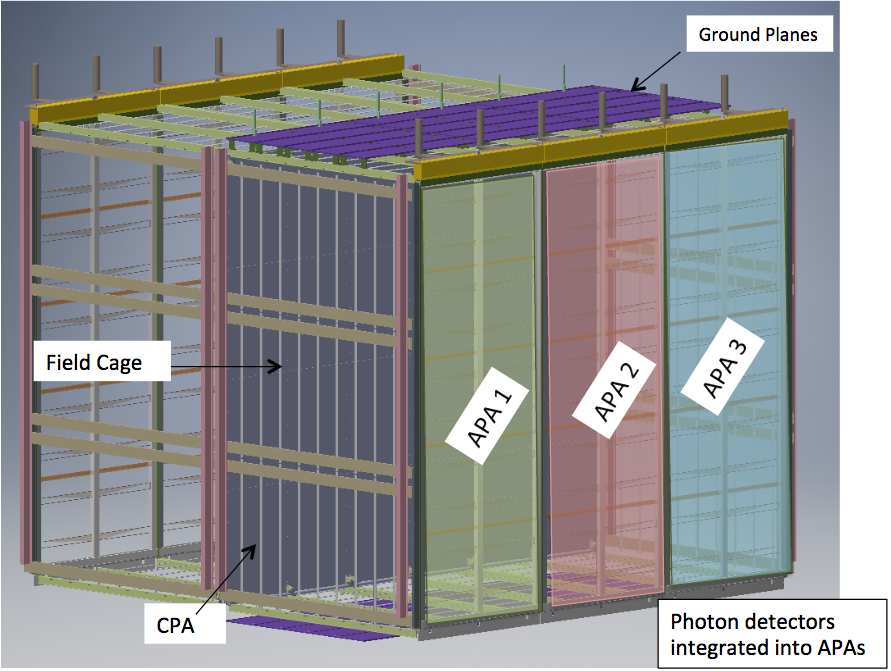
\includegraphics[width=0.9\textwidth]{protodune-sp-tpc-touramanis}
\end{cdrfigure}

The CE, mounted onto the APA frame, and thus immersed in LAr, amplifies and continuously digitizes the induced signals on the sense wires at several MHz, and transmits these waveforms to the Data Acquisition system (DAQ). From the DAQ the data are  transmitted through the buffer to disk, then to the central CERN Tier-0 Computing Center, and finally to other partner sites for processing and analysis.  

The modular PDS is integrated into the APAs. Each PDS module (referred to as a PD) consists of a bar-shaped light guide and
a wavelength-shifting layer (surface-coating or mounted radiator plate). The wavelength-shifting layer converts incoming VUV (128 nm) 
scintillation photons to longer-wavelength photons, in the visible blue range. Some of the converted photons are emitted into the bar, a fraction of which are then internally reflected to the bar's end where they are detected by silicon photomultipliers (SiPMs).
Each APA frame is designed with ten bays into which PDs are inserted after the TPC wires have been strung. This  allows for final assembly at the integration area (in a clean room) at the CERN NP prior to installation inside the cryostat. 


%%%%%%%%%%%%%%%%%%%%%%%%%%%%%%%%%%%%%%%%%%%%%%%%%%%%
\section{Goals of ProtoDUNE-SP}
\label{intro:goals}
ProtoDUNE-SP has four principal goals, all of which are essential parts of the DUNE far detector development program:
\begin{itemize}
\item Prototype the production and installation procedures for the single-phase far detector design.
\item Validate the design from the perspective of basic detector performance; this can be achieved with cosmic-ray data. 
This is the critical step from the perspective of establishing the design for the DUNE TDRs, which will undergo LBNC and DOE reviews in 2019.
\item Accumulate large samples of test-beam data to understand/calibrate the response of the detector to different particle species. 
\item Demonstrate the long-term operational stability of the detector as part of the risk mitigation program ahead of the construction of the first \ktadj{10} far detector module.
\end{itemize}
Commissioning and successfully bringing the detector into operation and maintaining it in a stable operating condition over a period of %the order of (1-3) - OK
one-to-three months would allow for validation of the design through a full characterization of the detector components, including the membrane cryostat and the cooling and purification circuit, the APA design and the layout of its cold read-out electronics, the HV system, and the PDS and its warm read-out electronics. This can be achieved by collecting cosmic-ray data. 

The large samples of test-beam data of different particle species would allow for a more in-depth understanding the response of the detector and could ultimately be used for calibration purposes. The analysis of the test-beam data will involve strong feedback 
between reconstruction, detector simulation, and hadronic modeling. Three types of systematic effects will be addressed: (1) a detailed understanding of energy scale and energy resolution for electromagnetic and hadronic showers; (2) the detector response to different particle species, including %measuring - OK
the impact of recombination effects as a function of angle; and (3) improved modeling of the interactions of hadrons in argon, which will provide constraints to the GEANT4 physics models.  A run period of approximately three months in the test beam is considered sufficient, assuming stable operation under good beam conditions. The aim is to accumulate these data before the start of LS2 (Jul-Oct, 2018). 

The liquid argon technology is, however, sufficiently new that it would be highly desirable to perform a long-term test of ProtoDUNE-SP, extending beyond the start of LS2, to reduce risks associated with the extended operation of the DUNE far detector modules. This argues for cosmic-ray operation in 2019 and most likely 2020. This extended running period would be an important component of our risk mitigation strategy for the overall DUNE detector construction effort. \fixme{construction not operation? - it is: construction}

%\fixme{(Anne) rewrite (check against orig below): }
%The idea here is that since ongoing studies are not completed yet (regarding the level at which systematics in DUNE oscillation measurements can be constrained through analysis of ProtoDUNE test-beam data) => the precise n. of event to take cannot be determined right now.  
%The other idea is that  in any case the n. of event to collect is NOT the driving reason for asking 3 months of beam (the main reason being to have time to test the detector functionality for a sufficiently long time - as said above). 
% The third idea here is that we cannot know whether the detector and/or the beamline will perform well (or not), so we want to keep open the possibility for a second run after LS2.

%In your revised sentence the order (n.of evts vs ongoing studies) is reversed, and 
% the sentence starting with "Although ... " is connected to the "actual detector performance .." 

%This is a quite sensitive sentence and the steps have to follow the ideas listed here - of course the way to express these can/should be improved

%New version (?):
Ongoing detailed studies aim to quantify estimates regarding the level at which systematics in DUNE oscillation measurements can be constrained through analysis of ProtoDUNE test-beam data. The precise number of beam events required to meet the DUNE oscillation analysis physics goals is not yet determined - but this is not the primary driver of the beam time request.
It should be noted that the run duration will depend heavily upon actual detector performance and the beam quality (i.e., precision in particle momentum, impact position, beam PID), and that large uncertainties will remain until both ProtoDUNE-SP and the H4 beamline are commissioned. For all these reasons, beam operation after LS2 cannot be excluded.

%Current:
%The precise number of beam events required to meet the DUNE oscillation analysis physics goals cannot yet be determined. Ongoing detailed studies aim to quantify estimates regarding the level at which systematics in DUNE oscillation measurements can be constrained through analysis of ProtoDUNE test-beam data. Although these measurements are not the primary driver of the beam time request, it should be noted that the run duration will depend heavily upon actual detector performance and the beam quality (i.e., precision in particle momentum, impact position, beam PID), and that large uncertainties will remain until both ProtoDUNE-SP and the H4 beamline are commissioned. For all these reasons, beam operation after LS2 cannot be excluded.

%Orig pgraph:
% Ongoing detailed studies aim to quantitative statements regarding the level at which systematics in DUNE oscillation measurements can be constrained through analysis of ProtoDUNE test-beam data. The precise number of beam events that are required to meet the DUNE oscillation analysis physics goals thus cannot be determined at this stage - but this it is not driving the beam time request. It should be noted that the run duration will heavily depend upon actual detector performance and the beam quality (precision in particle momentum, impact position, beam PID) and until the commissioning of both LArTPC detector and H4 beam-line, there will be large uncertainties. For all these reasons, beam operation after LS2 cannot be excluded.

%%%%%%%%%%%%%%%%%%%%
\subsection{Detector engineering validation}  

%One of the primary goals of the ProtoDUNE-SP experiment is to validate the engineering design of the elements proposed for the \ktadj{10}  DUNE-SP. 

ProtoDUNE-SP is designed such that it will provide information on the actual far detector performance in as close as possible a configuration to the actual far detector layout, given the practical considerations imposed by time, space, and cost. To achieve this, the cold components are identical to the components proposed for the far detector, to the extent possible. 

%As an example, the APA modules are full-scale pre-production modules for the far detector. The full-scale APA modules have 20 front-end readout board instrumenting each and 10 integrated photon detector paddles. The ground connections between the electronics, the APA mechanical structure, the photon detectors, and the detector support structure are the same as those proposed for DUNE SP detector. ProtoDUNE-SP is instrumented with three APAs along each wall; this will test for cross talk between the middle APA and its neighbors. However, some practical limitations have required compromise in the ProtoDUNE-SP design. The far detector is designed with a 12-m-high TPC, based on a two-APA-high layout in which the bottom APA is hung from the top APA. Given the space available and the cost of the cryogenics infrastructure, it is not practical to have a 12-m-high test experiment. For these reasons the ProtoDUNE-SP TPC is one APA high. The collaboration will test the mechanical process of installing the two-APA detector configuration, along with the related cabling, separately.
The APAs are full-scale pre-production modules for the far detector.  The ground connections between the electronics, the APA mechanical structure, the photon detectors, and the detector support structure are the same as those proposed for DUNE-SP. ProtoDUNE-SP is instrumented with three APAs along each wall; this will test for cross talk between the middle APA and its neighbors. Whereas DUNE-SP is designed with a 12-m-high TPC, based on a two-APA-high layout, ProtoDUNE-SP TPC is one APA high, due to practical limitations. The collaboration will test the mechanical process of installing the two-APA detector configuration, along with the related cabling, separately.

%Flavio
% Also here need to reorder things as before (eg the sentence "Since there is no charge amplification in the liquid, the electronics is required to be extremely sensitive." is connected to the discussion on grounding "The grounding and shielding are therefore critical"). 

%%%%%% begin new FLC:
 The cold readout electronics  is based on the DUNE-SP cryogenic front-end pre-amp/shaper chip and ADC design. The front-end ASIC is essentially the final design {%that will be used in the first DUNE-SP module - wouldnt say so as this is not decided yet}. 
while the cold ADC ASIC is not the final version and the dedicated ASIC (COLDATA) for serializing the data and providing a 1-GB/s link is not yet available. Given the schedule constraints for ProtoDUNE-SP, an FPGA that emulates the COLDATA functionality is used and mounted on a dedicated mezzanine board. % too much detail --; it is mounted on a dedicated mezzanine board. - Indeed, it is an important detail bcs it makes clear that it is added on top, and not replacing it or modifying the mother board}
All the analog components, the conversion to digital, and the grounding/power distribution for the final electronics can be tested in this configuration.  

%this sentence is crucial: it is not nice in English for sure -  but the message I think is clear - if you find ways to improve the language, will be great, otherwise would stay as is.
This configuration of the electronics chain is the only option for meeting the requirement for protoDUNE-SP data collection in 2018 (requirement set by the schedule for the major LBNC and DOE reviews of the DUNE TDR that will take place in 2019 and the need of validation of the basic TPC design by then).
In the event further optimization of the ASICs (ADC and COLDATA) is required based on the ProtoDUNE-SP findings, it can be implemented before the start of production in 2020. 

Since there is no charge amplification in the liquid, the electronics is required to be extremely sensitive. The grounding and shielding are therefore critical, and the designs are as similar as is practical to those of DUNE-SP. The building ground in ENH1, with the interconnected rebar in the concrete floor 
%all the rebar in the concrete floor interconnected and then this network 
connected to the building ground bus, will provide a fairly good ground. The cryostat itself is isolated from the building ground, and all the mechanical/electrical connections have dielectric breaks. DUNE-SP, in contrast, will be installed a mile underground in a very dry mine, and better isolation from the environment is expected. ProtoDUNE-SP will test the ground isolation and shielding under conservative conditions.
%%%%%% end new FLC


%%%%%% begin anne
%Since there is no charge amplification in the liquid, the electronics is required to be extremely sensitive. The cold readout electronics design is based on the DUNE-SP cryogenic front-end pre-amp/shaper chip and ADC.  The front-end ASIC design is essentially the final design that will be used in the first DUNE-SP module. However, the cold ADC ASIC is not the final version, and the dedicated ASIC (COLDATA) for serializing the data and providing a 1-GB/s link is not yet available. Given the schedule constraints for ProtoDUNE-SP, an FPGA that emulates its functionality will be used with the existing electronics chain. % too much detail --; it is mounted on a dedicated mezzanine board. - OK
%All the analog components, the conversion to digital, and the grounding/power distribution for the final electronics can be tested in this configuration.  In the event further optimization of the ASICs (ADC and COLDATA) is required based on the ProtoDUNE-SP findings, it can be implemented before the start of production in 2020. 

%The grounding and shielding are critical, and the designs are as similar as is practical to those of DUNE-SP. The building ground in ENH1, with the interconnected rebar in the concrete floor 
%all the rebar in the concrete floor interconnected and then this network 
%connected to the building ground bus, will provide a fairly good ground. The cryostat itself is isolated from the building ground, and all the mechanical/electrical connections have dielectric breaks. DUNE-SP, in contrast, will be installed a mile underground in a very dry mine, and better isolation from the environment is expected. ProtoDUNE-SP will test the ground isolation and shielding under conservative conditions.
%%%%%% end anne

%Flavio's original
%The cold readout electronics design is based on the DUNE-SP cryogenic front-end pre-amp/shaper chip and ADC.  The front-end ASIC is essentially the final design. However, the cold ADC ASIC is not the final version and the dedicated ASIC (COLDATA) for serializing the data and providing a 1-GB/s link is not yet available, therefore an FPGA emulating its functionality is used; it is mounted on a dedicated mezzanine board. All the analog components, the conversion to digital, and the grounding/power distribution for the final electronics can be tested in this configuration. 

%The timescale for the validation of the basic TPC design is driven by the schedule for the major LBNC and DOE reviews of the DUNE TDR that will take place in 2019. This sets the requirement for protoDUNE-SP data collection in 2018.  The existing electronics chain is the only option for meeting this requirement. In the event further optimization of the ASICs (ADC an COLDATA) is required based on the ProtoDUNE-SP findings, it can be implemented before the start of production in 2020. 

%Since there is no charge amplification in the liquid, the electronics is required to be extremely sensitive. The grounding and shielding are therefore critical, and the designs are as similar as is practical to those of DUNE-SP. The building ground in ENH1, with the interconnected rebar in the concrete floor connected to the building ground bus, will provide a fairly good ground. The cryostat itself is isolated from the building ground, and all the mechanical/electrical connections have dielectric breaks. DUNE-SP, in contrast, will be installed a mile underground in a very dry mine, and better isolation from the environment is expected. ProtoDUNE-SP will test the ground isolation and shielding under conservative conditions.
%%% end Flavio's orig

The FC and cathode planes are full-scale prototypes, 
%final far detector elements. As the ProtoDUNE-SP detector is designed with full-scale field cages 
%the maximum drift distance and corresponding high voltage will be the same as planned for the far detector. 
with the same maximum drift distance and corresponding high voltage.
This allows ProtoDUNE-SP to use the same HV feedthrough and drift-field configuration as is planned for DUNE-SP. The cryostat dimensions are selected to be the same for both ProtoDUNEs %as the Dual-Phase (DP) cryostat in order to only need to design one cryostat and cryogenics system. 
to leverage the same cryostat and cryogenics system designs. 
In order to fit the ProtoDUNE-SP TPC in the cryostat, the wall-to-cathode plane distance is slightly smaller than in DUNE-SP, making this setup a conservative test of the HV design. 
Testing the TPC components under the most likely operating conditions for DUNE-SP is extremely important, as this is the first test of the updated LArTPC design, which incorporates a resistive cathode 
and FC construction with metal profiles and fiberglass I-beam support. 

ProtoDUNE-SP also offers a unique platform to validate and possibly optimize the cryogenics design for DUNE-SP. 
All cryostat penetrations are designed with gas purge to prevent contaminates from migrating from warm surfaces to the ullage volume, and the the liquid and gas flows inside the cryostat are being modeled. This is expected to provide an excellent test bed to validate the cryogenics design for DUNE-SP. 

%The installation process has many similarities to the far detector installation but also many differences. Both installation plans now call for inserting the equipment through a TCO. ProtoDUNE-SP will prototype the tooling and procedures for transporting an APA and transferring it to a suspended rail system. Similarly, the assembly and transport processes of the cathode planes and top/bottom field cages will be developed. Neither the hanging of one APA from the other nor the of moving a 12-m-tall stacked module will be tested. Likewise, the CPA is only 6~m tall, not 12~m. One major change in the installation was driven by the need to install the end walls with the TCO closure and the beam interface. Due to the tight space inside the cryostat, the rail structure on which the detector is hung will most likely be different for the final detector. Despite these differences, the experience gained in installing the ProtoDUNE-SP detector will be invaluable in planning the DUNE far detector installation. 

ProtoDUNE-SP will prototype the tooling and procedures for transporting APAs and transferring them to a suspended rail system. Similarly, the assembly and transport processes of the CPAs and top/bottom FC assemblies are being developed.  Due to space constraints inside the cryostat, the rail structure on which the detector is hung will most likely be different for DUNE-SP. Despite these differences, the experience gained in installing the ProtoDUNE-SP detector will be invaluable in planning the DUNE-SP installation. 

%Finally, one significant difference between the ProtoDUNE-SP detector and DUNE-SP is the integration of the test beam. This requires a penetration into the cryostat and a LAr displacement plug that bridges the gap between the membrane cryostat wall and the FC. As this element bridges the HV, careful design is required. To ensure that the displacement plug does not compromise the ProtoDUNE-SP operation, a dedicated HV test at Fermilab is planned that will test the final beam plug in the exact field configuration planned for ProtoDUNE-SP.

Integration of the test beam with ProtoDUNE-SP is quite different from the neutrino beam integration planned for DUNE-SP. To minimize the material interactions of the particle beam in the ProtoDUNE-SP cryostat upstream of the TPC, a volume of LAr along the beam path (between the cryostat membrane and the FC) is displaced, and replaced by a less dense volume of dry nitrogen gas. This requires a penetration into one of the FC assemblies to install a  beam plug. To ensure that the displacement plug does not compromise the ProtoDUNE-SP operation, a dedicated HV test at Fermilab is planned that will test the final beam plug in the exact field configuration planned for ProtoDUNE-SP.




%%%%%%%%%%%%%%%%%%%%
\subsection{Physics}

The use of the CERN charged-particle beams of known particle type and incident energy provide the means to achieve a better understanding of the interaction processes occuring within a argon target and help to optimize event reconstruction techniques, particle identification algortihms, and calorimetric energy measurements.   
The beam measurements will also provide a calibration data set for tuning the Monte Carlo simulations and a reference data set for the DUNE experiment. 

Pion and proton beams in an energy range from about one to a few GeV will be used primarily to study hadronic interaction mechanisms and secondary particle production.  At higher energies, these beams will be used to study shower reconstruction and energy calibration. Electrons will be used to benchmark and tune electron/photon separation algorithms, to study electromagnetic cascade processes and to calibrate electromagnetic showers at higher energies. Charged kaons produced in the tertiary beamline are rare but are copiously produced by the pion beam interactions inside the detector. These will be extremely useful for characterizing kaon identification efficiency for proton decay sensitivity studies.  Samples of stopping muons with Michel electrons from muon decay (or without them, in the case of negative muon capture) will be used for energy calibrations in the low-energy range of the SN neutrino events and for the development of charge-sign determination methods. 

A cumulative ProtoDUNE-SP test-beam run period of 16 weeks is assumed, but it depends on the extent of beamline sharing with other users at EHN1. The run will take place prior to the long shutdown of the LHC in late 2018 (LS2). 

ProtoDUNE-SP will acquire cosmic data during periods with no beam. A dedicated external trigger system consisting of arrays of scintillator paddles, suitably positioned and arranged in \textit{coincidence} trigger logic, 
will select specific classes of cosmic muon events. Dedicated runs, e.g., runs looking for long muon tracks crossing the entire detector at large zenith angles, allow for an overall test of the detector performance and the DAQ. Runs looking for muons stopping inside the LAr volume and the accumulation of accurate Michel electron spectra may be useful for energy calibration purposes in the low-energy range.

It is important to note that ProtoDUNE-SP offers much beyond calibration  and detector performance characterization.  The LArTPC simultaneously features precise 3D tracking and accurate measurement of energy deposited. Its large active volume allows for good containment of the hadronic and electromagnetic interaction products in the few GeV range. These capabilities have never before been combined in one detector.  The unprecedented event reconstruction capability combined with the exposure of the detector's large active volume to the CERN charged-particle beams open the way to a truly rich program of new physics investigations into particle interaction processes. 

  Hadronic ($\pi$, K and $p$) interactions on an Ar target around one GeV produce low-multiplicity final states rather than ``hadron showers,'' and similarily 1-GeV electrons  (with critical energy $\simeq 30$ MeV in Ar) produce low-populated cascades, with only a few tens of secondary energetic electrons (positrons).
``TPC/imaging-aided calorimetric measurements'' will allow investigations of energy deposition mechanisms in this energy range where the standard hadronic and electromagnetic shower concepts and features are either not well defined or cannot be applied.
The calorimetric measurement of the total energy deposited can, in fact, be accomplished, by detecting and summing over the energy deposited by each individual secondary particle/track thanks to the imaging capabilities of the LArTPC.
In particular, the determination of the electromagnetic  content in hadron-initiated cascades, $\pi^0$ multiplicity, and the energy fraction carried as a function of primary hadron incident energy will be of interest.

%%%%%%%%%%%%%%%%%%%%%%%%%%%%%%%%%%%%%%%%%%%%%%
\section{Run plan}
\label{sec:runplan}

\fixme{May need some intro/transition content here since this section was just moved in from a different part of the document}

Beam simulations show that the hadron rates at 
energies below 1~GeV/c are low. Moreover, low-energy beams are more
subject to degradation by materials in the
beamline.  The optimization of the run plan factors in the beam composition and particle rates of the H4 beamline, and 
also particle interaction topologies in the ProtoDUNE-SP detector. Full 
simulations of particle transport in the ProtoDUNE-SP detector, including the
beam window, have been performed.


At a beam momentum of 1~GeV/c, 35\% of protons are stopped before reaching the active TPC region, while the percentage reduces to 0.5\% at 2~GeV/c.  The kinetic energy distributions of protons and pions at the entrance point of the TPC for different beam momenta are shown in Figure~\ref{fig:pandpiint}. 
The fraction of stopping $\pi$'s for one $\pi$
produced at the secondary target is 3\% at $p=0.4$~GeV/c and decreases to 1.3\% at $p=0.7$~GeV/c.
The long distance (37~m) between the secondary target and the front of the LAr cryostat has a significant impact on the pion and kaon rates in the TPC. Due to pion lifetime, many of the  low-energy pions produced at the secondary target decay in the beam pipe before reaching the cryostat. The situation is even more significant for kaons; most kaons below 2~Gev/c do not make it to the cryostat.
Consequently the H4 beamline will not be operated much below 1~GeV/c in the hadron mode.
For electrons, %we would want 
the beam momentum should go %to go 
as low as possible to study the topology of very low-energy electron-initiated 
showers.
\begin{cdrfigure}[Energy at interaction]{pandpiint}{Kinetic energy of
    particles at the point of interaction in the ProtoDUNE-SP active
    volume, for different beam momenta. Histograms are normalized to one particle injected in the
    beamline acceptance. Simulations include the beam window
    materials, beams are considered as monochromatic and
    parallel. Left: protons, Right: pions.}
  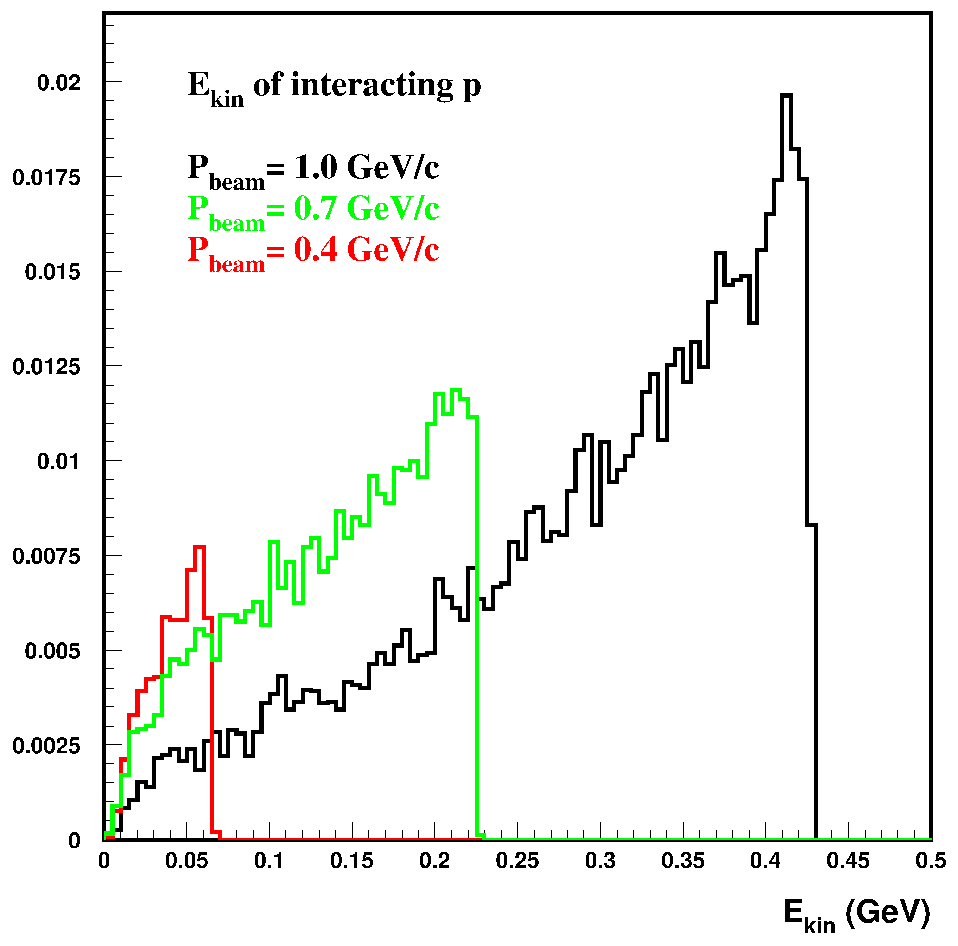
\includegraphics[width=0.49\textwidth]{pvarie_intene.pdf}
  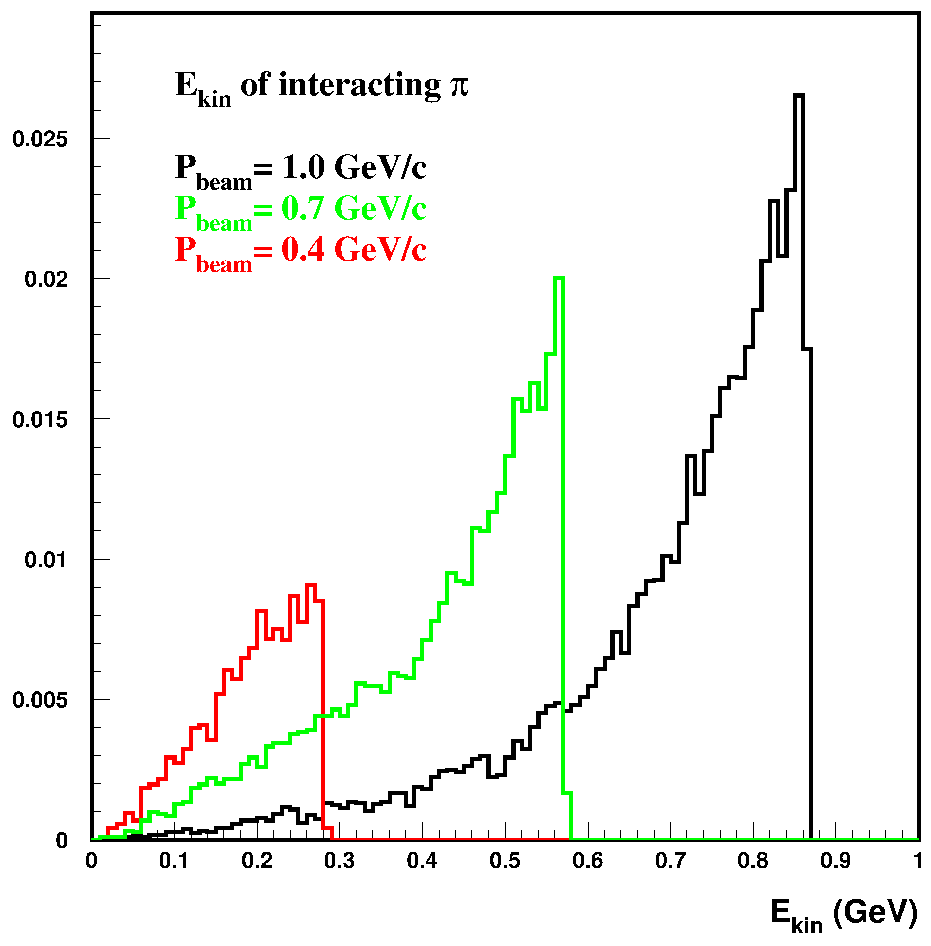
\includegraphics[width=0.49\textwidth]{pivarie_intene.pdf}
\end{cdrfigure}


To formulate a preliminary run plan, %we assume 
the hadron beam spectrum and rates are assumed as given in Tables~\ref{tab:beampartcomp} and~\ref{tab:beampartrates}.   For the purpose of estimating the sample composition and beam time request, the following assumptions are used:
\begin{itemize}
\item { Trigger rate = 25~Hz}
\item { Two 4.8 sec spills per SPS Super Cycle }
\item { SPS Super Cycle = 48 sec}
\item { $10^6$ ($10^4$) secondary particles on target per spill for hadron (electron) beam}
\item { Particle ID trigger for electrons from 0.5 to 7 GeV/c}
\item { Trigger rate for electron in hadron beam is prescaled to 0.5~Hz}
\item { Data collection efficiency = 50\%}
\end{itemize}

The question whether H2 and H4 tertiary beamlines at EHN1 can run simultaneously has not yet been resolved 
(to our knowledge). \fixme{(Anne) Seems like we should find out whether it's resolved yet. If not resolved I would say:} 

It has not yet been determined whether the H2 and H4 tertiary beamlines at EHN1 can run simultaneously, or 
%It is also not clear
 whether the secondary beam (upstream the target of the H4 beamline) will be shared with other users. Therefore, we have assumed a collection efficiency of 50\%. 
 \fixme{(Anne)If resolved, then restate accordingly.}

It is planned to run the H4 beamline in two modes: the first configuration is optimized for the production of hadrons and the second configuration is optimized for the production of high-purity electrons. Even in the hadron mode, the beam is still dominated by electrons, especially for low beam momenta. However, the electrons in the hadron beam are not particularly ``clean'' due to the amount of materials in the beamline from the particle identification (PID) instrumentations.  The proposal is to heavily prescale the electron events using PID (e.g., Threshold Cherenkov counters) trigger while running in hadron mode. The PID systems that contribute significantly to the material budget will be removed when %we reconfigure 
the beamline is reconfigured for electron beam.  Various run plan scenarios are under investigation. One of the scenarios is shown in Tables~\ref{tab:HadRunPlan} and ~\ref{tab:ElecRunPlan}. Similar values are expected for the negative beam sample. 
\begin{cdrtable}[Preliminary run plan for ProtoDUNE-SP hadron beam]{ccccccccc}{HadRunPlan}{A preliminary run plan for ProtoDUNE-S\
P hadron beam. The expected sample (positive beam) as a function of momentum is shown. }
P & \# of  &\# of $e^+$ & \# of $K^+$ & \# of $\mu^+$ & \# of $p$ & \# of $\pi^+$ & Total \# & Beam Time \\
(GeV/c) & Spills  & &  &  &  &  & of Events & (days) \\ \toprowrule
1 & 70K & 84K & $\approx$ 0 & 70K  & 689K & 625K & 1.5M & 19.4 days\\ \colhline
2 & 16K & 19K & 9K & 36K     & 336K & 572K & 1.0M &4.4 days\\ \colhline
3 & 13K & 16K & 26K  & 17K   & 181K & 540K  & 780K & 3.6 days\\ \colhline
4 & 11K & 13K & 19K & 16K    & 107K  & 510K & 660K & 3.1 days\\ \colhline
5 & 11K & 13K  & 29K  & 13K   & 96K  & 510K & 660K & 3.1 days\\ \colhline
6 & 11K & 13K & 36K  & 12K    & 94K  & 510K & 660K & 3.1 days\\ \colhline
7 & 11K & 13K & 42K & 8K     & 87K  & 510K & 660K & 3.1 days\\ \toprowrule
Total & 143K & 171K & 161K & 172K & 1.6M & 3.8M & 5.9M & 39.7 days\\
\end{cdrtable}
\begin{cdrtable}[Preliminary run plan for ProtoDUNE-SP electron beam]{cccc}{ElecRunPlan}{A preliminary run plan for ProtoDUNE-SP electron beam. The expected sample for positive beam configuration is shown. }
Momentum Bins & \# of Spills per Bin & \# $e^+$ per Bin & Beam Time per Bin \\ 
(GeV/c) & & & (days) \\ \toprowrule
0.5, 06, 0.7, 0.8, 0.9, 1, 2, 3, 4, 5, 6, 7 & 5000 & 300K & 1.4 \\
\end{cdrtable}

Based on the information available, the total estimated beam time needed to carry out the physics program in this proposal, with the assumptions stated earlier, is on the order of 16 weeks.
 
 



